\chapter{Evaluation}
\label{chapter:evaluation}

\section{Tests Objectives}

The test conducted were chosen because they have direct contribution with this thesis goals.

Our system leverages user detection to improve occupant comfort and reduce wasted energy and because of that we require the user detection to have medium/low accuracy in building detection time and high accuracy in room detection.



%In order to evaluate the developed system, several tests were performed. Section 5.1 starts by describing
%the test scenario. Next, in Section 5.2 the detailed description of each test is presented. Finally,
%Section 5.3 presents the results of the tests.

\section{Tests Scenarios}



All the tests were conducted in real scenarios inside a office of the IST - Taguspark campus. They
were executed using the hardware described in Section~\ref{hardware_arch_imp} and one Moto G3 phone running the user app.


\subsection{User detection - Room}


In order to test the reaction time of user detection in the office, a series of measurements were performed. The test consists in observing the time the user app takes to detect the Estimote beacon present inside the office (beacon with 3.5 meter range). The user will start walking from just outside the beacon range and walk normally to the office door.

The measurements will be performed with the beacon device near the door in order to increase signal range outside the office. The device used will be a Moto G3 Android phone with BT support up to version 4.0 .
For testing purposes the user app is set to vibrate when it near the beacon in order for us to know if it found the beacon, a chronometer will be used to determine the reaction time. The test will result in at least a set of 20 measurements in order to determine a meaningful average of the reaction time of the system.


\subsection{User detection - Building}

In order to test the reaction time of user detection in the building, a series of measurements were performed. The test consists in observing the time the user app takes to detect phone is inside the building. The user will start walking from the front door of the building to the office door.

The device used will be a Moto G3 Android phone with WiFi support.
For testing purposes the user app is set to vibrate when it is inside the building, a chronometer will be used to determine the reaction time. The test will result in at least a set of 20 measurements in order to determine a meaningful average of the reaction time of the system.



\subsection{Motion detection}

To test the motion detection a series of measurements were performed to test the algorithm. The test consists in a person walking in front of the Hub camera at different speeds from the door to a desk. This test will show if our system is able to detect motion when people enter the office and if it can be tricked and produce wrong negatives.




\subsection{Temperature and Luminosity}

This test measures the correct behavior of the built-in luminosity sensor and the external temperature sensor. 

The luminosity test consists in reading the sensor data in a room with no lights on, and then turn on the lights to determine if a change in the sensor was observed.

To test the temperature sensor the \ac{HVAC} system will be turned on, and the temperature readings will show if changes in temperature in the office were observed.


\subsection{Hub server load}

(stress test)

To test our system web-server a series of measures were performed. This test consists in making several concurrent \ac{HTTP} requests.

 concurring requests to our \ac{API} 


\subsection{Automation}

To evaluate the usability of the \ac{IFTT} interface (automation recipes), user usability tests were performed. The users who performed the tests were not familiar with our system and had no previous experience with similar \ac{IFTT} solutions.

The users were asked to create two distinct recipes:

\begin{itemize}
  \item If the user left the office, then tun off all the lights.
  \item If the temperature is above 25 ºC, then set temperature to below 20 ºC. 
\end{itemize} 

The test results were then compared to an expert user to determine the usability of the system.



\section{Test Results}


\subsection{User detection - Room}

A set of measurements were taken in order to determine the response time the application takes to identify the user's phone is inside the room. Two types of measurements were taken.

In the first the user is inside the room with \ac{BT} turned off, then it was turned on and timer started, column 1 of Table~\ref{eval:room} shows the measurements obtained. 

In the second set of measurements the user starts walking outside the office and opens a unlocked door to the room. The results for the second test are shown in column 2 of Table~\ref{eval:room}.

The mean median deviation for both tests are shown in Table~\ref{eval:room2}. We observed that in most cases our system detected the user presence very quickly within few seconds but in other occasions it seemed to take up to 30 seconds. We noticed once it detected the Estimote beacon it found it correctly the consecutive times but seems to take some time for the initial discovery. Looking at the second test, where the user enters the room, we see an average value 6 seconds and a standard deviation of 9 seconds. We consider the time to detect the user presence is adequate for turning on the \ac{HVAC} system in the user presence but not perfect for turning on the lights when the user enters the room.

For cases when the user wants the lights to be on when he enters the room and if the detection time is considered insufficient, a automation recipe can be created for turning on the light when movement is detected and the user is inside the building. Nevertheless we consider the room detection time adequate for rooms with ambient light from a window but not for dark rooms.

The office where the tests were conducted is roughly 3 by 10 meters wide. The Estimote beacon range was set to approximately 3.5 meters range. Regarding false positives the beacon signal can be observed in the adjacent office when next to the wall between the rooms. This means our system can incorrectly identifies the user presence when inside an adjacent office next to the wall. A possible solution to this problem is to use more than one beacon with range of 1.5 meters and spread them in the room. Since the range is shorter the signal won't be so easily detected in adjacent rooms but still offers coverage in the target room.


\begin{table}[]
\centering
\begin{tabular}{|r|r|}
\hline
\multicolumn{1}{|c|}{Test 1} & \multicolumn{1}{c|}{Test 2} \\
\multicolumn{1}{|l|}{\begin{tabular}[c]{@{}l@{}}Time (seconds) to detect user \\ presence in room, when user \\ is already inside\end{tabular}} & \multicolumn{1}{l|}{\begin{tabular}[c]{@{}l@{}}Time (seconds) to detect user \\ presence in room, when user \\ is outside and walks inside\end{tabular}} \\ \hline
2.13 & 7.63 \\ \hline
2.23 & 3.20 \\ \hline
2.02 & 18.70 \\ \hline
23.55 & 27.76 \\ \hline
6.65 & 24.26 \\ \hline
11.5 & 2.46 \\ \hline
7.16 & 0.91 \\ \hline
2.36 & 0.42 \\ \hline
2.18 & 22.62 \\ \hline
2.48 & 0.62 \\ \hline
12.4 & 1.12 \\ \hline
2.15 & 10.45 \\ \hline
6.73 & 16.63 \\ \hline
2.18 & 0 \\ \hline
11.93 & 0.26 \\ \hline
2.22 & 0.25 \\ \hline
2.12 & 19.28 \\ \hline
16.62 & 7.43 \\ \hline
2.08 & 12.83 \\ \hline
2.23 & 9.38 \\ \hline
\end{tabular}
\caption{Room detection measurements}
\label{eval:room}
\end{table}


\begin{table}[]
\centering
\begin{tabular}{l|r|r|}
\cline{2-3}
 & \multicolumn{1}{l|}{Test 1 (s)} & \multicolumn{1}{l|}{Test 2 (s)} \\ \hline
\multicolumn{1}{|l|}{Mean} & 6.14 & 9.31 \\ \hline
\multicolumn{1}{|l|}{Standard deviation} & 5.92 & 9.03 \\ \hline
\end{tabular}
\caption{Room detection  - Mean and Standard deviation for tests when the user is inside and walks inside the room}
\label{eval:room2}
\end{table}





\subsection{User detection - Building}

Several measurements were taken to determine the response time the application takes to identify the user is inside the building, these measurements are shown in Table~\ref{eval:building1}.

Building user detection does not need very quick response time unlike room detection, building location will be mostly used to preheat the room before the user arrives. The response time observed shows a acceptable response time with mean and standard deviation shown in Table~\ref{eval:building2}.



Our building \ac{WiFi} range extends a few meters beyond the front door so in some measurements our system detected the user before he walked to the front door of the building.







\begin{table}[]
\centering
\begin{tabular}{|l|}
\hline
Time (seconds) \\ \hline
21.44 \\ \hline
40.54 \\ \hline
0 \\ \hline
5.55 \\ \hline
30.23 \\ \hline
10.12 \\ \hline
0 \\ \hline
5.54 \\ \hline
34.12 \\ \hline
8.14 \\ \hline
0 \\ \hline
22.43 \\ \hline
45.32 \\ \hline
50.65 \\ \hline
26.24 \\ \hline
31.43 \\ \hline
45.76 \\ \hline
13.65 \\ \hline
17.43 \\ \hline
23.87 \\ \hline
\end{tabular}
\caption{User building detection, the time to detect the user starting in the building front door}
\label{eval:building1}
\end{table}

\begin{table}[]
\centering
\begin{tabular}{l|r|}
\cline{2-2}
 & \multicolumn{1}{l|}{Test 1} \\ \hline
\multicolumn{1}{|l|}{Mean} & 21.62 \\ \hline
\multicolumn{1}{|l|}{Median deviation} & 15.83 \\ \hline
\end{tabular}
\caption{Building detection  - Mean and Standard deviation for user detection time}
\label{eval:building2}
\end{table}



\subsection{Motion detection}

To test our motion detection algorithm and system, we conducted tests with three different people with different heights. Each person entered the room at different speeds, the obtained results are shown in Table~\ref{eval:motion}.

Our system was able to correctly identify a person walking inside the room every time, Figure~\ref{eval:motion_fig} shows the different pixels in the camera frames identified by our algorithm. Regarding false positives, they don't seem to be a problem since our system allow the creation of a no monitoring area in the camera frame to use in cases of rooms with window view.


\begin{table}[]
\centering
\begin{tabular}{|l|l|l|l|}
\hline
 & \begin{tabular}[c]{@{}l@{}}Person 1\\ detection\end{tabular} & \begin{tabular}[c]{@{}l@{}}Person 2\\ detection\end{tabular} & \begin{tabular}[c]{@{}l@{}}Person 3\\ detection\end{tabular} \\ \hline
Slow walk & 20/20 & 20/20 & 20/20 \\ \hline
Normal walk & 20/20 & 20/20 & 20/20 \\ \hline
Run & 20/20 & 20/20 & 20/20 \\ \hline
\end{tabular}
\caption{Motion detection tests for three people with different heights, 20 measurements each.}
\label{eval:motion}
\end{table}


\begin{figure}[h]
\centering
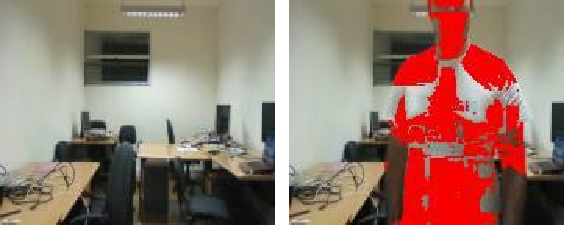
\includegraphics[width=0.4\textwidth]{Figures/eval_motion}
\caption{Motion detection - Frame before and after, motion detected }
\label{eval:motion_fig}
\end{figure}



\subsection{Temperature and Luminosity}











\subsection{Automation}

The results obtain from the usability test allow us to determine if further changes are need to improve our \ac{IFTT} interface. The test results are shown in  Table~\ref{eval:automation1}. We observed the users took more time completing the first task due to inexperience with the system, then they performed much better on the second task. 

One of the reasons user took more time in the first task was because after they correctly selected the trigger, they had to select an option inside the trigger, some options are not visible in the screen and the user needs to swipe vertically to show the remaining options.

Tests with an expert user were performed in order to compare the times of experienced and inexperience users when handling the interface. Comparing the results presented in Table~\ref{eval:automation2} and Table~\ref{eval:automation3} we observe the an inexperienced user on average took more 19 seconds to complete the first task in comparison with the experienced user. On average the inexperienced user took more 9 seconds to complete the second task.


\begin{table}[]
\centering
\begin{tabular}{|l|l|}
\hline
Task 1 & Task 2 \\ \hline
56 & 40 \\ \hline
23 & 24 \\ \hline
33 & 29 \\ \hline
41 & 26 \\ \hline
25 & 27 \\ \hline
28 & 22 \\ \hline
30 & 20 \\ \hline
24 & 20 \\ \hline
41 & 30 \\ \hline
35 & 27 \\ \hline
43 & 32 \\ \hline
34 & 20 \\ \hline
27 & 23 \\ \hline
36 & 29 \\ \hline
48 & 38 \\ \hline
35 & 28 \\ \hline
33 & 29 \\ \hline
55 & 40 \\ \hline
38 & 29 \\ \hline
35 & 23 \\ \hline
\end{tabular}
\caption{User usability tests results for task 1 and 2}
\label{eval:automation1}
\end{table}

\begin{table}[]
\centering
\begin{tabular}{l|r|r|}
\cline{2-3}
 & \multicolumn{1}{l|}{Task 1} & \multicolumn{1}{l|}{Task 2} \\ \hline
\multicolumn{1}{|l|}{Mean} & 36 & 27.8 \\ \hline
\multicolumn{1}{|l|}{Standard deviation} & 9.31 & 5.96 \\ \hline
\end{tabular}
\caption{User usability tests, mean and standard deviation}
\label{eval:automation2}
\end{table}


\begin{table}[]
\centering
\begin{tabular}{l|r|r|}
\cline{2-3}
 & \multicolumn{1}{l|}{Task 1} & \multicolumn{1}{l|}{Task 2} \\ \hline
\multicolumn{1}{|l|}{Mean} & 17 & 18.4 \\ \hline
\multicolumn{1}{|l|}{Standard deviation} & 0.89 & 1.49 \\ \hline
\end{tabular}
\caption{Expert user usability tests, mean and standard deviation}
\label{eval:automation3}
\end{table}


